% Created by tikzDevice version 0.12.3.1 on 2022-08-31 08:51:20
% !TEX encoding = UTF-8 Unicode
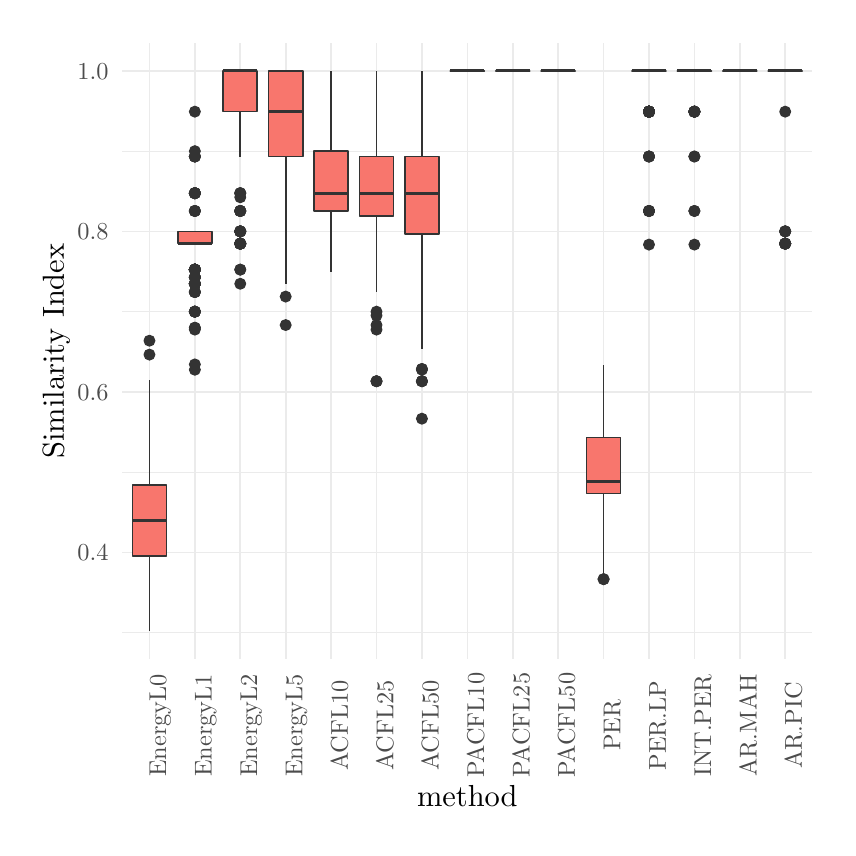
\begin{tikzpicture}[x=1pt,y=1pt]
\definecolor{fillColor}{RGB}{255,255,255}
\path[use as bounding box,fill=fillColor,fill opacity=0.00] (0,0) rectangle (289.08,289.08);
\begin{scope}
\path[clip] ( 34.16, 60.92) rectangle (283.58,283.58);
\definecolor{drawColor}{gray}{0.92}

\path[draw=drawColor,line width= 0.3pt,line join=round] ( 34.16, 70.45) --
	(283.58, 70.45);

\path[draw=drawColor,line width= 0.3pt,line join=round] ( 34.16,128.45) --
	(283.58,128.45);

\path[draw=drawColor,line width= 0.3pt,line join=round] ( 34.16,186.46) --
	(283.58,186.46);

\path[draw=drawColor,line width= 0.3pt,line join=round] ( 34.16,244.46) --
	(283.58,244.46);

\path[draw=drawColor,line width= 0.6pt,line join=round] ( 34.16, 99.45) --
	(283.58, 99.45);

\path[draw=drawColor,line width= 0.6pt,line join=round] ( 34.16,157.46) --
	(283.58,157.46);

\path[draw=drawColor,line width= 0.6pt,line join=round] ( 34.16,215.46) --
	(283.58,215.46);

\path[draw=drawColor,line width= 0.6pt,line join=round] ( 34.16,273.46) --
	(283.58,273.46);

\path[draw=drawColor,line width= 0.6pt,line join=round] ( 44.00, 60.92) --
	( 44.00,283.58);

\path[draw=drawColor,line width= 0.6pt,line join=round] ( 60.41, 60.92) --
	( 60.41,283.58);

\path[draw=drawColor,line width= 0.6pt,line join=round] ( 76.82, 60.92) --
	( 76.82,283.58);

\path[draw=drawColor,line width= 0.6pt,line join=round] ( 93.23, 60.92) --
	( 93.23,283.58);

\path[draw=drawColor,line width= 0.6pt,line join=round] (109.64, 60.92) --
	(109.64,283.58);

\path[draw=drawColor,line width= 0.6pt,line join=round] (126.05, 60.92) --
	(126.05,283.58);

\path[draw=drawColor,line width= 0.6pt,line join=round] (142.46, 60.92) --
	(142.46,283.58);

\path[draw=drawColor,line width= 0.6pt,line join=round] (158.87, 60.92) --
	(158.87,283.58);

\path[draw=drawColor,line width= 0.6pt,line join=round] (175.28, 60.92) --
	(175.28,283.58);

\path[draw=drawColor,line width= 0.6pt,line join=round] (191.69, 60.92) --
	(191.69,283.58);

\path[draw=drawColor,line width= 0.6pt,line join=round] (208.10, 60.92) --
	(208.10,283.58);

\path[draw=drawColor,line width= 0.6pt,line join=round] (224.51, 60.92) --
	(224.51,283.58);

\path[draw=drawColor,line width= 0.6pt,line join=round] (240.92, 60.92) --
	(240.92,283.58);

\path[draw=drawColor,line width= 0.6pt,line join=round] (257.32, 60.92) --
	(257.32,283.58);

\path[draw=drawColor,line width= 0.6pt,line join=round] (273.73, 60.92) --
	(273.73,283.58);
\definecolor{drawColor}{gray}{0.20}
\definecolor{fillColor}{gray}{0.20}

\path[draw=drawColor,line width= 0.4pt,line join=round,line cap=round,fill=fillColor] ( 44.00,175.97) circle (  1.96);

\path[draw=drawColor,line width= 0.4pt,line join=round,line cap=round,fill=fillColor] ( 44.00,170.94) circle (  1.96);

\path[draw=drawColor,line width= 0.6pt,line join=round] ( 44.00,123.87) -- ( 44.00,161.60);

\path[draw=drawColor,line width= 0.6pt,line join=round] ( 44.00, 98.12) -- ( 44.00, 71.04);
\definecolor{fillColor}{RGB}{248,118,109}

\path[draw=drawColor,line width= 0.6pt,line join=round,line cap=round,fill=fillColor] ( 37.85,123.87) --
	( 37.85, 98.12) --
	( 50.16, 98.12) --
	( 50.16,123.87) --
	( 37.85,123.87) --
	cycle;

\path[draw=drawColor,line width= 1.1pt,line join=round] ( 37.85,111.05) -- ( 50.16,111.05);
\definecolor{fillColor}{gray}{0.20}

\path[draw=drawColor,line width= 0.4pt,line join=round,line cap=round,fill=fillColor] ( 60.41,167.40) circle (  1.96);

\path[draw=drawColor,line width= 0.4pt,line join=round,line cap=round,fill=fillColor] ( 60.41,201.65) circle (  1.96);

\path[draw=drawColor,line width= 0.4pt,line join=round,line cap=round,fill=fillColor] ( 60.41,201.65) circle (  1.96);

\path[draw=drawColor,line width= 0.4pt,line join=round,line cap=round,fill=fillColor] ( 60.41,196.54) circle (  1.96);

\path[draw=drawColor,line width= 0.4pt,line join=round,line cap=round,fill=fillColor] ( 60.41,229.27) circle (  1.96);

\path[draw=drawColor,line width= 0.4pt,line join=round,line cap=round,fill=fillColor] ( 60.41,198.89) circle (  1.96);

\path[draw=drawColor,line width= 0.4pt,line join=round,line cap=round,fill=fillColor] ( 60.41,222.84) circle (  1.96);

\path[draw=drawColor,line width= 0.4pt,line join=round,line cap=round,fill=fillColor] ( 60.41,229.27) circle (  1.96);

\path[draw=drawColor,line width= 0.4pt,line join=round,line cap=round,fill=fillColor] ( 60.41,196.54) circle (  1.96);

\path[draw=drawColor,line width= 0.4pt,line join=round,line cap=round,fill=fillColor] ( 60.41,258.73) circle (  1.96);

\path[draw=drawColor,line width= 0.4pt,line join=round,line cap=round,fill=fillColor] ( 60.41,201.65) circle (  1.96);

\path[draw=drawColor,line width= 0.4pt,line join=round,line cap=round,fill=fillColor] ( 60.41,201.65) circle (  1.96);

\path[draw=drawColor,line width= 0.4pt,line join=round,line cap=round,fill=fillColor] ( 60.41,242.52) circle (  1.96);

\path[draw=drawColor,line width= 0.4pt,line join=round,line cap=round,fill=fillColor] ( 60.41,201.65) circle (  1.96);

\path[draw=drawColor,line width= 0.4pt,line join=round,line cap=round,fill=fillColor] ( 60.41,201.65) circle (  1.96);

\path[draw=drawColor,line width= 0.4pt,line join=round,line cap=round,fill=fillColor] ( 60.41,196.54) circle (  1.96);

\path[draw=drawColor,line width= 0.4pt,line join=round,line cap=round,fill=fillColor] ( 60.41,186.46) circle (  1.96);

\path[draw=drawColor,line width= 0.4pt,line join=round,line cap=round,fill=fillColor] ( 60.41,229.27) circle (  1.96);

\path[draw=drawColor,line width= 0.4pt,line join=round,line cap=round,fill=fillColor] ( 60.41,229.27) circle (  1.96);

\path[draw=drawColor,line width= 0.4pt,line join=round,line cap=round,fill=fillColor] ( 60.41,186.46) circle (  1.96);

\path[draw=drawColor,line width= 0.4pt,line join=round,line cap=round,fill=fillColor] ( 60.41,196.54) circle (  1.96);

\path[draw=drawColor,line width= 0.4pt,line join=round,line cap=round,fill=fillColor] ( 60.41,201.65) circle (  1.96);

\path[draw=drawColor,line width= 0.4pt,line join=round,line cap=round,fill=fillColor] ( 60.41,244.46) circle (  1.96);

\path[draw=drawColor,line width= 0.4pt,line join=round,line cap=round,fill=fillColor] ( 60.41,242.52) circle (  1.96);

\path[draw=drawColor,line width= 0.4pt,line join=round,line cap=round,fill=fillColor] ( 60.41,201.65) circle (  1.96);

\path[draw=drawColor,line width= 0.4pt,line join=round,line cap=round,fill=fillColor] ( 60.41,198.89) circle (  1.96);

\path[draw=drawColor,line width= 0.4pt,line join=round,line cap=round,fill=fillColor] ( 60.41,201.65) circle (  1.96);

\path[draw=drawColor,line width= 0.4pt,line join=round,line cap=round,fill=fillColor] ( 60.41,222.84) circle (  1.96);

\path[draw=drawColor,line width= 0.4pt,line join=round,line cap=round,fill=fillColor] ( 60.41,196.54) circle (  1.96);

\path[draw=drawColor,line width= 0.4pt,line join=round,line cap=round,fill=fillColor] ( 60.41,198.89) circle (  1.96);

\path[draw=drawColor,line width= 0.4pt,line join=round,line cap=round,fill=fillColor] ( 60.41,196.54) circle (  1.96);

\path[draw=drawColor,line width= 0.4pt,line join=round,line cap=round,fill=fillColor] ( 60.41,196.54) circle (  1.96);

\path[draw=drawColor,line width= 0.4pt,line join=round,line cap=round,fill=fillColor] ( 60.41,193.55) circle (  1.96);

\path[draw=drawColor,line width= 0.4pt,line join=round,line cap=round,fill=fillColor] ( 60.41,222.84) circle (  1.96);

\path[draw=drawColor,line width= 0.4pt,line join=round,line cap=round,fill=fillColor] ( 60.41,198.89) circle (  1.96);

\path[draw=drawColor,line width= 0.4pt,line join=round,line cap=round,fill=fillColor] ( 60.41,179.97) circle (  1.96);

\path[draw=drawColor,line width= 0.4pt,line join=round,line cap=round,fill=fillColor] ( 60.41,186.46) circle (  1.96);

\path[draw=drawColor,line width= 0.4pt,line join=round,line cap=round,fill=fillColor] ( 60.41,201.65) circle (  1.96);

\path[draw=drawColor,line width= 0.4pt,line join=round,line cap=round,fill=fillColor] ( 60.41,186.46) circle (  1.96);

\path[draw=drawColor,line width= 0.4pt,line join=round,line cap=round,fill=fillColor] ( 60.41,196.54) circle (  1.96);

\path[draw=drawColor,line width= 0.4pt,line join=round,line cap=round,fill=fillColor] ( 60.41,242.52) circle (  1.96);

\path[draw=drawColor,line width= 0.4pt,line join=round,line cap=round,fill=fillColor] ( 60.41,186.46) circle (  1.96);

\path[draw=drawColor,line width= 0.4pt,line join=round,line cap=round,fill=fillColor] ( 60.41,201.65) circle (  1.96);

\path[draw=drawColor,line width= 0.4pt,line join=round,line cap=round,fill=fillColor] ( 60.41,193.55) circle (  1.96);

\path[draw=drawColor,line width= 0.4pt,line join=round,line cap=round,fill=fillColor] ( 60.41,198.89) circle (  1.96);

\path[draw=drawColor,line width= 0.4pt,line join=round,line cap=round,fill=fillColor] ( 60.41,193.55) circle (  1.96);

\path[draw=drawColor,line width= 0.4pt,line join=round,line cap=round,fill=fillColor] ( 60.41,229.27) circle (  1.96);

\path[draw=drawColor,line width= 0.4pt,line join=round,line cap=round,fill=fillColor] ( 60.41,229.27) circle (  1.96);

\path[draw=drawColor,line width= 0.4pt,line join=round,line cap=round,fill=fillColor] ( 60.41,165.47) circle (  1.96);

\path[draw=drawColor,line width= 0.4pt,line join=round,line cap=round,fill=fillColor] ( 60.41,196.54) circle (  1.96);

\path[draw=drawColor,line width= 0.4pt,line join=round,line cap=round,fill=fillColor] ( 60.41,242.52) circle (  1.96);

\path[draw=drawColor,line width= 0.4pt,line join=round,line cap=round,fill=fillColor] ( 60.41,201.65) circle (  1.96);

\path[draw=drawColor,line width= 0.4pt,line join=round,line cap=round,fill=fillColor] ( 60.41,196.54) circle (  1.96);

\path[draw=drawColor,line width= 0.4pt,line join=round,line cap=round,fill=fillColor] ( 60.41,186.46) circle (  1.96);

\path[draw=drawColor,line width= 0.4pt,line join=round,line cap=round,fill=fillColor] ( 60.41,201.65) circle (  1.96);

\path[draw=drawColor,line width= 0.4pt,line join=round,line cap=round,fill=fillColor] ( 60.41,198.89) circle (  1.96);

\path[draw=drawColor,line width= 0.4pt,line join=round,line cap=round,fill=fillColor] ( 60.41,201.65) circle (  1.96);

\path[draw=drawColor,line width= 0.4pt,line join=round,line cap=round,fill=fillColor] ( 60.41,222.84) circle (  1.96);

\path[draw=drawColor,line width= 0.4pt,line join=round,line cap=round,fill=fillColor] ( 60.41,201.65) circle (  1.96);

\path[draw=drawColor,line width= 0.4pt,line join=round,line cap=round,fill=fillColor] ( 60.41,229.27) circle (  1.96);

\path[draw=drawColor,line width= 0.4pt,line join=round,line cap=round,fill=fillColor] ( 60.41,196.54) circle (  1.96);

\path[draw=drawColor,line width= 0.4pt,line join=round,line cap=round,fill=fillColor] ( 60.41,193.55) circle (  1.96);

\path[draw=drawColor,line width= 0.4pt,line join=round,line cap=round,fill=fillColor] ( 60.41,201.65) circle (  1.96);

\path[draw=drawColor,line width= 0.4pt,line join=round,line cap=round,fill=fillColor] ( 60.41,180.66) circle (  1.96);

\path[draw=drawColor,line width= 0.4pt,line join=round,line cap=round,fill=fillColor] ( 60.41,229.27) circle (  1.96);

\path[draw=drawColor,line width= 0.4pt,line join=round,line cap=round,fill=fillColor] ( 60.41,180.66) circle (  1.96);

\path[draw=drawColor,line width= 0.4pt,line join=round,line cap=round,fill=fillColor] ( 60.41,201.65) circle (  1.96);

\path[draw=drawColor,line width= 0.6pt,line join=round] ( 60.41,215.46) -- ( 60.41,215.46);

\path[draw=drawColor,line width= 0.6pt,line join=round] ( 60.41,211.04) -- ( 60.41,211.04);
\definecolor{fillColor}{RGB}{248,118,109}

\path[draw=drawColor,line width= 0.6pt,line join=round,line cap=round,fill=fillColor] ( 54.26,215.46) --
	( 54.26,211.04) --
	( 66.56,211.04) --
	( 66.56,215.46) --
	( 54.26,215.46) --
	cycle;

\path[draw=drawColor,line width= 1.1pt,line join=round] ( 54.26,211.04) -- ( 66.56,211.04);
\definecolor{fillColor}{gray}{0.20}

\path[draw=drawColor,line width= 0.4pt,line join=round,line cap=round,fill=fillColor] ( 76.82,229.27) circle (  1.96);

\path[draw=drawColor,line width= 0.4pt,line join=round,line cap=round,fill=fillColor] ( 76.82,211.04) circle (  1.96);

\path[draw=drawColor,line width= 0.4pt,line join=round,line cap=round,fill=fillColor] ( 76.82,201.65) circle (  1.96);

\path[draw=drawColor,line width= 0.4pt,line join=round,line cap=round,fill=fillColor] ( 76.82,215.46) circle (  1.96);

\path[draw=drawColor,line width= 0.4pt,line join=round,line cap=round,fill=fillColor] ( 76.82,196.54) circle (  1.96);

\path[draw=drawColor,line width= 0.4pt,line join=round,line cap=round,fill=fillColor] ( 76.82,222.84) circle (  1.96);

\path[draw=drawColor,line width= 0.4pt,line join=round,line cap=round,fill=fillColor] ( 76.82,211.04) circle (  1.96);

\path[draw=drawColor,line width= 0.4pt,line join=round,line cap=round,fill=fillColor] ( 76.82,211.04) circle (  1.96);

\path[draw=drawColor,line width= 0.4pt,line join=round,line cap=round,fill=fillColor] ( 76.82,215.46) circle (  1.96);

\path[draw=drawColor,line width= 0.4pt,line join=round,line cap=round,fill=fillColor] ( 76.82,215.46) circle (  1.96);

\path[draw=drawColor,line width= 0.4pt,line join=round,line cap=round,fill=fillColor] ( 76.82,211.04) circle (  1.96);

\path[draw=drawColor,line width= 0.4pt,line join=round,line cap=round,fill=fillColor] ( 76.82,201.65) circle (  1.96);

\path[draw=drawColor,line width= 0.4pt,line join=round,line cap=round,fill=fillColor] ( 76.82,222.84) circle (  1.96);

\path[draw=drawColor,line width= 0.4pt,line join=round,line cap=round,fill=fillColor] ( 76.82,215.46) circle (  1.96);

\path[draw=drawColor,line width= 0.4pt,line join=round,line cap=round,fill=fillColor] ( 76.82,222.84) circle (  1.96);

\path[draw=drawColor,line width= 0.4pt,line join=round,line cap=round,fill=fillColor] ( 76.82,215.46) circle (  1.96);

\path[draw=drawColor,line width= 0.4pt,line join=round,line cap=round,fill=fillColor] ( 76.82,229.27) circle (  1.96);

\path[draw=drawColor,line width= 0.4pt,line join=round,line cap=round,fill=fillColor] ( 76.82,222.84) circle (  1.96);

\path[draw=drawColor,line width= 0.4pt,line join=round,line cap=round,fill=fillColor] ( 76.82,211.04) circle (  1.96);

\path[draw=drawColor,line width= 0.4pt,line join=round,line cap=round,fill=fillColor] ( 76.82,215.46) circle (  1.96);

\path[draw=drawColor,line width= 0.4pt,line join=round,line cap=round,fill=fillColor] ( 76.82,227.79) circle (  1.96);

\path[draw=drawColor,line width= 0.4pt,line join=round,line cap=round,fill=fillColor] ( 76.82,211.04) circle (  1.96);

\path[draw=drawColor,line width= 0.4pt,line join=round,line cap=round,fill=fillColor] ( 76.82,211.04) circle (  1.96);

\path[draw=drawColor,line width= 0.4pt,line join=round,line cap=round,fill=fillColor] ( 76.82,222.84) circle (  1.96);

\path[draw=drawColor,line width= 0.4pt,line join=round,line cap=round,fill=fillColor] ( 76.82,215.46) circle (  1.96);

\path[draw=drawColor,line width= 0.4pt,line join=round,line cap=round,fill=fillColor] ( 76.82,211.04) circle (  1.96);

\path[draw=drawColor,line width= 0.4pt,line join=round,line cap=round,fill=fillColor] ( 76.82,211.04) circle (  1.96);

\path[draw=drawColor,line width= 0.4pt,line join=round,line cap=round,fill=fillColor] ( 76.82,211.04) circle (  1.96);

\path[draw=drawColor,line width= 0.4pt,line join=round,line cap=round,fill=fillColor] ( 76.82,222.84) circle (  1.96);

\path[draw=drawColor,line width= 0.4pt,line join=round,line cap=round,fill=fillColor] ( 76.82,229.27) circle (  1.96);

\path[draw=drawColor,line width= 0.4pt,line join=round,line cap=round,fill=fillColor] ( 76.82,211.04) circle (  1.96);

\path[draw=drawColor,line width= 0.6pt,line join=round] ( 76.82,273.46) -- ( 76.82,273.46);

\path[draw=drawColor,line width= 0.6pt,line join=round] ( 76.82,258.73) -- ( 76.82,242.52);
\definecolor{fillColor}{RGB}{248,118,109}

\path[draw=drawColor,line width= 0.6pt,line join=round,line cap=round,fill=fillColor] ( 70.67,273.46) --
	( 70.67,258.73) --
	( 82.97,258.73) --
	( 82.97,273.46) --
	( 70.67,273.46) --
	cycle;

\path[draw=drawColor,line width= 1.1pt,line join=round] ( 70.67,273.46) -- ( 82.97,273.46);
\definecolor{fillColor}{gray}{0.20}

\path[draw=drawColor,line width= 0.4pt,line join=round,line cap=round,fill=fillColor] ( 93.23,181.62) circle (  1.96);

\path[draw=drawColor,line width= 0.4pt,line join=round,line cap=round,fill=fillColor] ( 93.23,191.91) circle (  1.96);

\path[draw=drawColor,line width= 0.6pt,line join=round] ( 93.23,273.46) -- ( 93.23,273.46);

\path[draw=drawColor,line width= 0.6pt,line join=round] ( 93.23,242.52) -- ( 93.23,196.54);
\definecolor{fillColor}{RGB}{248,118,109}

\path[draw=drawColor,line width= 0.6pt,line join=round,line cap=round,fill=fillColor] ( 87.08,273.46) --
	( 87.08,242.52) --
	( 99.38,242.52) --
	( 99.38,273.46) --
	( 87.08,273.46) --
	cycle;

\path[draw=drawColor,line width= 1.1pt,line join=round] ( 87.08,258.73) -- ( 99.38,258.73);

\path[draw=drawColor,line width= 0.6pt,line join=round] (109.64,244.46) -- (109.64,273.46);

\path[draw=drawColor,line width= 0.6pt,line join=round] (109.64,222.84) -- (109.64,200.73);

\path[draw=drawColor,line width= 0.6pt,line join=round,line cap=round,fill=fillColor] (103.49,244.46) --
	(103.49,222.84) --
	(115.79,222.84) --
	(115.79,244.46) --
	(103.49,244.46) --
	cycle;

\path[draw=drawColor,line width= 1.1pt,line join=round] (103.49,229.27) -- (115.79,229.27);
\definecolor{fillColor}{gray}{0.20}

\path[draw=drawColor,line width= 0.4pt,line join=round,line cap=round,fill=fillColor] (126.05,185.08) circle (  1.96);

\path[draw=drawColor,line width= 0.4pt,line join=round,line cap=round,fill=fillColor] (126.05,186.46) circle (  1.96);

\path[draw=drawColor,line width= 0.4pt,line join=round,line cap=round,fill=fillColor] (126.05,161.32) circle (  1.96);

\path[draw=drawColor,line width= 0.4pt,line join=round,line cap=round,fill=fillColor] (126.05,161.32) circle (  1.96);

\path[draw=drawColor,line width= 0.4pt,line join=round,line cap=round,fill=fillColor] (126.05,179.97) circle (  1.96);

\path[draw=drawColor,line width= 0.4pt,line join=round,line cap=round,fill=fillColor] (126.05,161.32) circle (  1.96);

\path[draw=drawColor,line width= 0.4pt,line join=round,line cap=round,fill=fillColor] (126.05,181.62) circle (  1.96);

\path[draw=drawColor,line width= 0.6pt,line join=round] (126.05,242.52) -- (126.05,273.46);

\path[draw=drawColor,line width= 0.6pt,line join=round] (126.05,220.99) -- (126.05,193.55);
\definecolor{fillColor}{RGB}{248,118,109}

\path[draw=drawColor,line width= 0.6pt,line join=round,line cap=round,fill=fillColor] (119.90,242.52) --
	(119.90,220.99) --
	(132.20,220.99) --
	(132.20,242.52) --
	(119.90,242.52) --
	cycle;

\path[draw=drawColor,line width= 1.1pt,line join=round] (119.90,229.27) -- (132.20,229.27);
\definecolor{fillColor}{gray}{0.20}

\path[draw=drawColor,line width= 0.4pt,line join=round,line cap=round,fill=fillColor] (142.46,165.74) circle (  1.96);

\path[draw=drawColor,line width= 0.4pt,line join=round,line cap=round,fill=fillColor] (142.46,147.79) circle (  1.96);

\path[draw=drawColor,line width= 0.4pt,line join=round,line cap=round,fill=fillColor] (142.46,161.32) circle (  1.96);

\path[draw=drawColor,line width= 0.4pt,line join=round,line cap=round,fill=fillColor] (142.46,161.32) circle (  1.96);

\path[draw=drawColor,line width= 0.4pt,line join=round,line cap=round,fill=fillColor] (142.46,165.47) circle (  1.96);

\path[draw=drawColor,line width= 0.4pt,line join=round,line cap=round,fill=fillColor] (142.46,161.32) circle (  1.96);

\path[draw=drawColor,line width= 0.4pt,line join=round,line cap=round,fill=fillColor] (142.46,165.74) circle (  1.96);

\path[draw=drawColor,line width= 0.6pt,line join=round] (142.46,242.52) -- (142.46,273.46);

\path[draw=drawColor,line width= 0.6pt,line join=round] (142.46,214.54) -- (142.46,172.92);
\definecolor{fillColor}{RGB}{248,118,109}

\path[draw=drawColor,line width= 0.6pt,line join=round,line cap=round,fill=fillColor] (136.31,242.52) --
	(136.31,214.54) --
	(148.61,214.54) --
	(148.61,242.52) --
	(136.31,242.52) --
	cycle;

\path[draw=drawColor,line width= 1.1pt,line join=round] (136.31,229.27) -- (148.61,229.27);

\path[draw=drawColor,line width= 0.6pt,line join=round] (158.87,273.46) -- (158.87,273.46);

\path[draw=drawColor,line width= 0.6pt,line join=round] (158.87,273.46) -- (158.87,273.46);

\path[draw=drawColor,line width= 0.6pt,line join=round,line cap=round,fill=fillColor] (152.71,273.46) --
	(152.71,273.46) --
	(165.02,273.46) --
	(165.02,273.46) --
	(152.71,273.46) --
	cycle;

\path[draw=drawColor,line width= 1.1pt,line join=round] (152.71,273.46) -- (165.02,273.46);

\path[draw=drawColor,line width= 0.6pt,line join=round] (175.28,273.46) -- (175.28,273.46);

\path[draw=drawColor,line width= 0.6pt,line join=round] (175.28,273.46) -- (175.28,273.46);

\path[draw=drawColor,line width= 0.6pt,line join=round,line cap=round,fill=fillColor] (169.12,273.46) --
	(169.12,273.46) --
	(181.43,273.46) --
	(181.43,273.46) --
	(169.12,273.46) --
	cycle;

\path[draw=drawColor,line width= 1.1pt,line join=round] (169.12,273.46) -- (181.43,273.46);

\path[draw=drawColor,line width= 0.6pt,line join=round] (191.69,273.46) -- (191.69,273.46);

\path[draw=drawColor,line width= 0.6pt,line join=round] (191.69,273.46) -- (191.69,273.46);

\path[draw=drawColor,line width= 0.6pt,line join=round,line cap=round,fill=fillColor] (185.53,273.46) --
	(185.53,273.46) --
	(197.84,273.46) --
	(197.84,273.46) --
	(185.53,273.46) --
	cycle;

\path[draw=drawColor,line width= 1.1pt,line join=round] (185.53,273.46) -- (197.84,273.46);
\definecolor{fillColor}{gray}{0.20}

\path[draw=drawColor,line width= 0.4pt,line join=round,line cap=round,fill=fillColor] (208.10, 89.79) circle (  1.96);

\path[draw=drawColor,line width= 0.4pt,line join=round,line cap=round,fill=fillColor] (208.10, 89.79) circle (  1.96);

\path[draw=drawColor,line width= 0.6pt,line join=round] (208.10,141.02) -- (208.10,167.12);

\path[draw=drawColor,line width= 0.6pt,line join=round] (208.10,120.72) -- (208.10, 91.95);
\definecolor{fillColor}{RGB}{248,118,109}

\path[draw=drawColor,line width= 0.6pt,line join=round,line cap=round,fill=fillColor] (201.94,141.02) --
	(201.94,120.72) --
	(214.25,120.72) --
	(214.25,141.02) --
	(201.94,141.02) --
	cycle;

\path[draw=drawColor,line width= 1.1pt,line join=round] (201.94,125.14) -- (214.25,125.14);
\definecolor{fillColor}{gray}{0.20}

\path[draw=drawColor,line width= 0.4pt,line join=round,line cap=round,fill=fillColor] (224.51,222.84) circle (  1.96);

\path[draw=drawColor,line width= 0.4pt,line join=round,line cap=round,fill=fillColor] (224.51,258.73) circle (  1.96);

\path[draw=drawColor,line width= 0.4pt,line join=round,line cap=round,fill=fillColor] (224.51,258.73) circle (  1.96);

\path[draw=drawColor,line width= 0.4pt,line join=round,line cap=round,fill=fillColor] (224.51,258.73) circle (  1.96);

\path[draw=drawColor,line width= 0.4pt,line join=round,line cap=round,fill=fillColor] (224.51,258.73) circle (  1.96);

\path[draw=drawColor,line width= 0.4pt,line join=round,line cap=round,fill=fillColor] (224.51,258.73) circle (  1.96);

\path[draw=drawColor,line width= 0.4pt,line join=round,line cap=round,fill=fillColor] (224.51,242.52) circle (  1.96);

\path[draw=drawColor,line width= 0.4pt,line join=round,line cap=round,fill=fillColor] (224.51,222.84) circle (  1.96);

\path[draw=drawColor,line width= 0.4pt,line join=round,line cap=round,fill=fillColor] (224.51,258.73) circle (  1.96);

\path[draw=drawColor,line width= 0.4pt,line join=round,line cap=round,fill=fillColor] (224.51,258.73) circle (  1.96);

\path[draw=drawColor,line width= 0.4pt,line join=round,line cap=round,fill=fillColor] (224.51,258.73) circle (  1.96);

\path[draw=drawColor,line width= 0.4pt,line join=round,line cap=round,fill=fillColor] (224.51,258.73) circle (  1.96);

\path[draw=drawColor,line width= 0.4pt,line join=round,line cap=round,fill=fillColor] (224.51,258.73) circle (  1.96);

\path[draw=drawColor,line width= 0.4pt,line join=round,line cap=round,fill=fillColor] (224.51,242.52) circle (  1.96);

\path[draw=drawColor,line width= 0.4pt,line join=round,line cap=round,fill=fillColor] (224.51,258.73) circle (  1.96);

\path[draw=drawColor,line width= 0.4pt,line join=round,line cap=round,fill=fillColor] (224.51,258.73) circle (  1.96);

\path[draw=drawColor,line width= 0.4pt,line join=round,line cap=round,fill=fillColor] (224.51,258.73) circle (  1.96);

\path[draw=drawColor,line width= 0.4pt,line join=round,line cap=round,fill=fillColor] (224.51,258.73) circle (  1.96);

\path[draw=drawColor,line width= 0.4pt,line join=round,line cap=round,fill=fillColor] (224.51,258.73) circle (  1.96);

\path[draw=drawColor,line width= 0.4pt,line join=round,line cap=round,fill=fillColor] (224.51,258.73) circle (  1.96);

\path[draw=drawColor,line width= 0.4pt,line join=round,line cap=round,fill=fillColor] (224.51,258.73) circle (  1.96);

\path[draw=drawColor,line width= 0.4pt,line join=round,line cap=round,fill=fillColor] (224.51,222.84) circle (  1.96);

\path[draw=drawColor,line width= 0.4pt,line join=round,line cap=round,fill=fillColor] (224.51,258.73) circle (  1.96);

\path[draw=drawColor,line width= 0.4pt,line join=round,line cap=round,fill=fillColor] (224.51,242.52) circle (  1.96);

\path[draw=drawColor,line width= 0.4pt,line join=round,line cap=round,fill=fillColor] (224.51,258.73) circle (  1.96);

\path[draw=drawColor,line width= 0.4pt,line join=round,line cap=round,fill=fillColor] (224.51,258.73) circle (  1.96);

\path[draw=drawColor,line width= 0.4pt,line join=round,line cap=round,fill=fillColor] (224.51,258.73) circle (  1.96);

\path[draw=drawColor,line width= 0.4pt,line join=round,line cap=round,fill=fillColor] (224.51,258.73) circle (  1.96);

\path[draw=drawColor,line width= 0.4pt,line join=round,line cap=round,fill=fillColor] (224.51,258.73) circle (  1.96);

\path[draw=drawColor,line width= 0.4pt,line join=round,line cap=round,fill=fillColor] (224.51,222.84) circle (  1.96);

\path[draw=drawColor,line width= 0.4pt,line join=round,line cap=round,fill=fillColor] (224.51,210.69) circle (  1.96);

\path[draw=drawColor,line width= 0.4pt,line join=round,line cap=round,fill=fillColor] (224.51,258.73) circle (  1.96);

\path[draw=drawColor,line width= 0.4pt,line join=round,line cap=round,fill=fillColor] (224.51,258.73) circle (  1.96);

\path[draw=drawColor,line width= 0.4pt,line join=round,line cap=round,fill=fillColor] (224.51,258.73) circle (  1.96);

\path[draw=drawColor,line width= 0.4pt,line join=round,line cap=round,fill=fillColor] (224.51,258.73) circle (  1.96);

\path[draw=drawColor,line width= 0.4pt,line join=round,line cap=round,fill=fillColor] (224.51,242.52) circle (  1.96);

\path[draw=drawColor,line width= 0.4pt,line join=round,line cap=round,fill=fillColor] (224.51,258.73) circle (  1.96);

\path[draw=drawColor,line width= 0.4pt,line join=round,line cap=round,fill=fillColor] (224.51,222.84) circle (  1.96);

\path[draw=drawColor,line width= 0.6pt,line join=round] (224.51,273.46) -- (224.51,273.46);

\path[draw=drawColor,line width= 0.6pt,line join=round] (224.51,273.46) -- (224.51,273.46);
\definecolor{fillColor}{RGB}{248,118,109}

\path[draw=drawColor,line width= 0.6pt,line join=round,line cap=round,fill=fillColor] (218.35,273.46) --
	(218.35,273.46) --
	(230.66,273.46) --
	(230.66,273.46) --
	(218.35,273.46) --
	cycle;

\path[draw=drawColor,line width= 1.1pt,line join=round] (218.35,273.46) -- (230.66,273.46);
\definecolor{fillColor}{gray}{0.20}

\path[draw=drawColor,line width= 0.4pt,line join=round,line cap=round,fill=fillColor] (240.92,210.69) circle (  1.96);

\path[draw=drawColor,line width= 0.4pt,line join=round,line cap=round,fill=fillColor] (240.92,242.52) circle (  1.96);

\path[draw=drawColor,line width= 0.4pt,line join=round,line cap=round,fill=fillColor] (240.92,258.73) circle (  1.96);

\path[draw=drawColor,line width= 0.4pt,line join=round,line cap=round,fill=fillColor] (240.92,258.73) circle (  1.96);

\path[draw=drawColor,line width= 0.4pt,line join=round,line cap=round,fill=fillColor] (240.92,222.84) circle (  1.96);

\path[draw=drawColor,line width= 0.4pt,line join=round,line cap=round,fill=fillColor] (240.92,258.73) circle (  1.96);

\path[draw=drawColor,line width= 0.4pt,line join=round,line cap=round,fill=fillColor] (240.92,222.84) circle (  1.96);

\path[draw=drawColor,line width= 0.4pt,line join=round,line cap=round,fill=fillColor] (240.92,258.73) circle (  1.96);

\path[draw=drawColor,line width= 0.4pt,line join=round,line cap=round,fill=fillColor] (240.92,258.73) circle (  1.96);

\path[draw=drawColor,line width= 0.4pt,line join=round,line cap=round,fill=fillColor] (240.92,258.73) circle (  1.96);

\path[draw=drawColor,line width= 0.4pt,line join=round,line cap=round,fill=fillColor] (240.92,242.52) circle (  1.96);

\path[draw=drawColor,line width= 0.4pt,line join=round,line cap=round,fill=fillColor] (240.92,258.73) circle (  1.96);

\path[draw=drawColor,line width= 0.4pt,line join=round,line cap=round,fill=fillColor] (240.92,258.73) circle (  1.96);

\path[draw=drawColor,line width= 0.4pt,line join=round,line cap=round,fill=fillColor] (240.92,258.73) circle (  1.96);

\path[draw=drawColor,line width= 0.6pt,line join=round] (240.92,273.46) -- (240.92,273.46);

\path[draw=drawColor,line width= 0.6pt,line join=round] (240.92,273.46) -- (240.92,273.46);
\definecolor{fillColor}{RGB}{248,118,109}

\path[draw=drawColor,line width= 0.6pt,line join=round,line cap=round,fill=fillColor] (234.76,273.46) --
	(234.76,273.46) --
	(247.07,273.46) --
	(247.07,273.46) --
	(234.76,273.46) --
	cycle;

\path[draw=drawColor,line width= 1.1pt,line join=round] (234.76,273.46) -- (247.07,273.46);

\path[draw=drawColor,line width= 0.6pt,line join=round] (257.32,273.46) -- (257.32,273.46);

\path[draw=drawColor,line width= 0.6pt,line join=round] (257.32,273.46) -- (257.32,273.46);

\path[draw=drawColor,line width= 0.6pt,line join=round,line cap=round,fill=fillColor] (251.17,273.46) --
	(251.17,273.46) --
	(263.48,273.46) --
	(263.48,273.46) --
	(251.17,273.46) --
	cycle;

\path[draw=drawColor,line width= 1.1pt,line join=round] (251.17,273.46) -- (263.48,273.46);
\definecolor{fillColor}{gray}{0.20}

\path[draw=drawColor,line width= 0.4pt,line join=round,line cap=round,fill=fillColor] (273.73,211.04) circle (  1.96);

\path[draw=drawColor,line width= 0.4pt,line join=round,line cap=round,fill=fillColor] (273.73,211.04) circle (  1.96);

\path[draw=drawColor,line width= 0.4pt,line join=round,line cap=round,fill=fillColor] (273.73,211.04) circle (  1.96);

\path[draw=drawColor,line width= 0.4pt,line join=round,line cap=round,fill=fillColor] (273.73,211.04) circle (  1.96);

\path[draw=drawColor,line width= 0.4pt,line join=round,line cap=round,fill=fillColor] (273.73,211.04) circle (  1.96);

\path[draw=drawColor,line width= 0.4pt,line join=round,line cap=round,fill=fillColor] (273.73,215.46) circle (  1.96);

\path[draw=drawColor,line width= 0.4pt,line join=round,line cap=round,fill=fillColor] (273.73,215.46) circle (  1.96);

\path[draw=drawColor,line width= 0.4pt,line join=round,line cap=round,fill=fillColor] (273.73,258.73) circle (  1.96);

\path[draw=drawColor,line width= 0.4pt,line join=round,line cap=round,fill=fillColor] (273.73,215.46) circle (  1.96);

\path[draw=drawColor,line width= 0.4pt,line join=round,line cap=round,fill=fillColor] (273.73,211.04) circle (  1.96);

\path[draw=drawColor,line width= 0.4pt,line join=round,line cap=round,fill=fillColor] (273.73,215.46) circle (  1.96);

\path[draw=drawColor,line width= 0.4pt,line join=round,line cap=round,fill=fillColor] (273.73,211.04) circle (  1.96);

\path[draw=drawColor,line width= 0.4pt,line join=round,line cap=round,fill=fillColor] (273.73,211.04) circle (  1.96);

\path[draw=drawColor,line width= 0.6pt,line join=round] (273.73,273.46) -- (273.73,273.46);

\path[draw=drawColor,line width= 0.6pt,line join=round] (273.73,273.46) -- (273.73,273.46);
\definecolor{fillColor}{RGB}{248,118,109}

\path[draw=drawColor,line width= 0.6pt,line join=round,line cap=round,fill=fillColor] (267.58,273.46) --
	(267.58,273.46) --
	(279.89,273.46) --
	(279.89,273.46) --
	(267.58,273.46) --
	cycle;

\path[draw=drawColor,line width= 1.1pt,line join=round] (267.58,273.46) -- (279.89,273.46);
\end{scope}
\begin{scope}
\path[clip] (  0.00,  0.00) rectangle (289.08,289.08);
\definecolor{drawColor}{gray}{0.30}

\node[text=drawColor,anchor=base east,inner sep=0pt, outer sep=0pt, scale=  0.88] at ( 29.21, 96.42) {0.4};

\node[text=drawColor,anchor=base east,inner sep=0pt, outer sep=0pt, scale=  0.88] at ( 29.21,154.43) {0.6};

\node[text=drawColor,anchor=base east,inner sep=0pt, outer sep=0pt, scale=  0.88] at ( 29.21,212.43) {0.8};

\node[text=drawColor,anchor=base east,inner sep=0pt, outer sep=0pt, scale=  0.88] at ( 29.21,270.43) {1.0};
\end{scope}
\begin{scope}
\path[clip] (  0.00,  0.00) rectangle (289.08,289.08);
\definecolor{drawColor}{gray}{0.30}

\node[text=drawColor,rotate= 90.00,anchor=base,inner sep=0pt, outer sep=0pt, scale=  0.88] at ( 50.06, 36.97) {EnergyL0};

\node[text=drawColor,rotate= 90.00,anchor=base,inner sep=0pt, outer sep=0pt, scale=  0.88] at ( 66.47, 36.97) {EnergyL1};

\node[text=drawColor,rotate= 90.00,anchor=base,inner sep=0pt, outer sep=0pt, scale=  0.88] at ( 82.88, 36.97) {EnergyL2};

\node[text=drawColor,rotate= 90.00,anchor=base,inner sep=0pt, outer sep=0pt, scale=  0.88] at ( 99.29, 36.97) {EnergyL5};

\node[text=drawColor,rotate= 90.00,anchor=base,inner sep=0pt, outer sep=0pt, scale=  0.88] at (115.70, 36.97) {ACFL10};

\node[text=drawColor,rotate= 90.00,anchor=base,inner sep=0pt, outer sep=0pt, scale=  0.88] at (132.11, 36.97) {ACFL25};

\node[text=drawColor,rotate= 90.00,anchor=base,inner sep=0pt, outer sep=0pt, scale=  0.88] at (148.52, 36.97) {ACFL50};

\node[text=drawColor,rotate= 90.00,anchor=base,inner sep=0pt, outer sep=0pt, scale=  0.88] at (164.93, 36.97) {PACFL10};

\node[text=drawColor,rotate= 90.00,anchor=base,inner sep=0pt, outer sep=0pt, scale=  0.88] at (181.34, 36.97) {PACFL25};

\node[text=drawColor,rotate= 90.00,anchor=base,inner sep=0pt, outer sep=0pt, scale=  0.88] at (197.75, 36.97) {PACFL50};

\node[text=drawColor,rotate= 90.00,anchor=base,inner sep=0pt, outer sep=0pt, scale=  0.88] at (214.16, 36.97) {PER};

\node[text=drawColor,rotate= 90.00,anchor=base,inner sep=0pt, outer sep=0pt, scale=  0.88] at (230.57, 36.97) {PER.LP};

\node[text=drawColor,rotate= 90.00,anchor=base,inner sep=0pt, outer sep=0pt, scale=  0.88] at (246.98, 36.97) {INT.PER};

\node[text=drawColor,rotate= 90.00,anchor=base,inner sep=0pt, outer sep=0pt, scale=  0.88] at (263.39, 36.97) {AR.MAH};

\node[text=drawColor,rotate= 90.00,anchor=base,inner sep=0pt, outer sep=0pt, scale=  0.88] at (279.80, 36.97) {AR.PIC};
\end{scope}
\begin{scope}
\path[clip] (  0.00,  0.00) rectangle (289.08,289.08);
\definecolor{drawColor}{RGB}{0,0,0}

\node[text=drawColor,anchor=base,inner sep=0pt, outer sep=0pt, scale=  1.10] at (158.87,  7.64) {method};
\end{scope}
\begin{scope}
\path[clip] (  0.00,  0.00) rectangle (289.08,289.08);
\definecolor{drawColor}{RGB}{0,0,0}

\node[text=drawColor,rotate= 90.00,anchor=base,inner sep=0pt, outer sep=0pt, scale=  1.10] at ( 13.08,172.25) {Similarity Index};
\end{scope}
\end{tikzpicture}
